\clearpage
\chapter{Markt} \label{KapitelMarkt}
\section{Aufbau}
(TH) Der Markt stellt die zentrale Einheit dar, die die für jede einzelne Angebotene Uhr die abgenommene Menge bestimmt. Dabei gelten folgende Vorgaben und Annahmen.
\begin{enumerate}
	\item Der Markt soll in drei Marktsegmente unterteilt sein
	\\ Entsprechend der drei Uhrenkategorien soll auch der Markt in drei Segmente geteilt sein, die größtenteils getrennt voneinander agieren.
	\item Jeder Markt soll jedem Spieler die gleichen Möglichkeiten bieten.
	\\ Um jedem Spieler, unabhängig von der Wahl seines Urtyps, die Chance auf den Sieg zu geben sollen die 3 Teilmärkte, in die der Markt gegliedert, jeweils das gleiche Volumen besitzen. Dies ist zwar nicht realitätsgetreu, verhindert jedoch ein zu langweiliges Spiel.
	\item Die Uhren sollen sich je nach Preis und Ausstattung unterschiedlich gut verkaufen
	\\ Die durch den Markt simulierten Konsumenten sollen nicht einfach nur blind nach ihrem Budgetkaufen, sondern schlechte Angebote unterschiedlich stark nachfragen.
	\item Die drei Marktsegmente sollen sich gegenseitig beeinflussen
	\\ Jede Uhr soll die Möglichkeit haben, die Anderen zu beeinflussen, auch wenn diese in anderen Marktsegmenten positioniert sind.
	\item Die Uhren im selben Marktsegment sollen sich gegenseitig beeinflussen
	\\ Uhren im selben Preissegment und mit ähnlichen Preisen konkurrieren um die selben Kunden, dies muss sich auch in den Verkaufszahlen wiederspiegeln.
\end{enumerate}

Die genaue Implementierung des Marktes lässt sich auch in diese Unterpunkte unterteilen. Dazu wird von den anderen Teilen der Unternehmenssimulation erwartet, dass jeder Spieler, ein Objekt der Klasse /enquote{/texttt{Unternehmen}} ist. Diese werden beim Starten der Marktsimulation als Array übergeben und besitzen wiederum ein Array an Uhren. Jede Uhr hat alle benötigten Attribute, um die Simulation durchzuführen, wie die offensichtlich benötigten Werte Angebotspreis, angebotene Menge und Marktsegment. Als zusätzlichen Parameter muss der Uhr noch einen Wert zugewiesen werden. Dieser spiegelt wieder, dass Uhren mit besseren Uhrwerken, Gehäusen oder Armbändern auch zu teureren Verkaufspreisen angeboten werden können. Daher ist dieser Wert angelehnt an die Entwicklung dieser Attribute und die daraus resultierende Produktionskostensteigerung. Der Marktwert wird automatisch beim Verbessern der Uhren aktualisiert und steht immer in jeder einzelnen Uhr zur Verfügung. Die komplette Marktsimulation kann mit diesen Werten ausgeführt werden.

\begin{enumerate}
	\item Der Markt soll in drei Marktsegmente unterteilt sein
	\\ Die Unterteilung des Marktes in die einzelnen Marktsegmente wird über eine Instanz der Klasse \enquote{\texttt{Gesamtmarkt}} verwaltet, die intern über je eine Instanz der Klasse \enquote{\texttt{Teilmarkt}} für jedes Segment verfügt. Diese werden zu Beginn, beim Erstellen des Marktes, automatisch mit dem im \texttt{Gesamtmarkt}-Konstruktor mitgegebenen Parametern gleichermaßen erstellt.
	\item Jeder Markt soll jedem Spieler die gleichen Möglichkeiten bieten.
	\\ Dem \texttt{Gesamtmarkt}, und damit den Teilmärkten, wird ein \enquote{\texttt{volume}} übergeben. Dieser Wert kann als Umsatz zu jedem Preis über das gesamte Preisspektrum erreicht werden. Die Formel zur Berechnung des Marktvolumens in Stückzahlen zu einem bestimmten Preis lautet demnach: \(Marktvolumen(Preis)=volume/Preis\).
	\item Die Uhren sollen sich je nach Preis und Ausstattung unterschiedlich gut verkaufen
	\\ Für die Simulation dieser Anforderung wurde angenommen, dass ein Konsument ein begrenztes Budget besitzt. Nach seinen Budgetvorstellungen versucht er nun eine Uhr zu kaufen, bevorzugt dabei aber natürlich besser ausgestattete Uhren bzw. Uhren mit besserem Preis-Leistungs-Verhältnis. Dazu wird in den Uhrenklassen eine Abnahmequote berechnet. Diese soll eine spätere Bevorzugung von preislich aggressiveren Angeboten bei gleichzeitiger Benachteiligung von überteuerten Angeboten ermöglichen. \\
	Der erste Schritt dabei stellte die Abbildung des Preis-Leistungs-Verhältnisses, das Werte im Bereich \([0;\infty]\) und das ausgeglichene Verhältnis bei \(1\) auf eine nicht-logarithmische Skala. Dies hat die Aufgabe, das z.\,B. ein Verhältnis von \(2:1\) den gleichen Wert wie ein Verhältnis von \(1:2\) bekommt, nur mit unterschiedlichen Vorzeichen, was durch folgende Funktion erreicht wird: \[\frac{2,5*\log (\frac{Preis}{Marktwert})}{log 2}\]
	Um diesen Wert nun wieder auf ein Quote mit Werten im Bereich \([0;1]\) abzubilden, wurde diese Funktion wiederum mit einem logistischen Wachstum kombiniert, wie in der nächsten Formel zu sehen. \[\frac{1}{1+e^{\frac{2,5*\log (\frac{Preis}{Marktwert})}{log 2}}} \]\\
	
	\begin{figure}[!h]
		\centering
		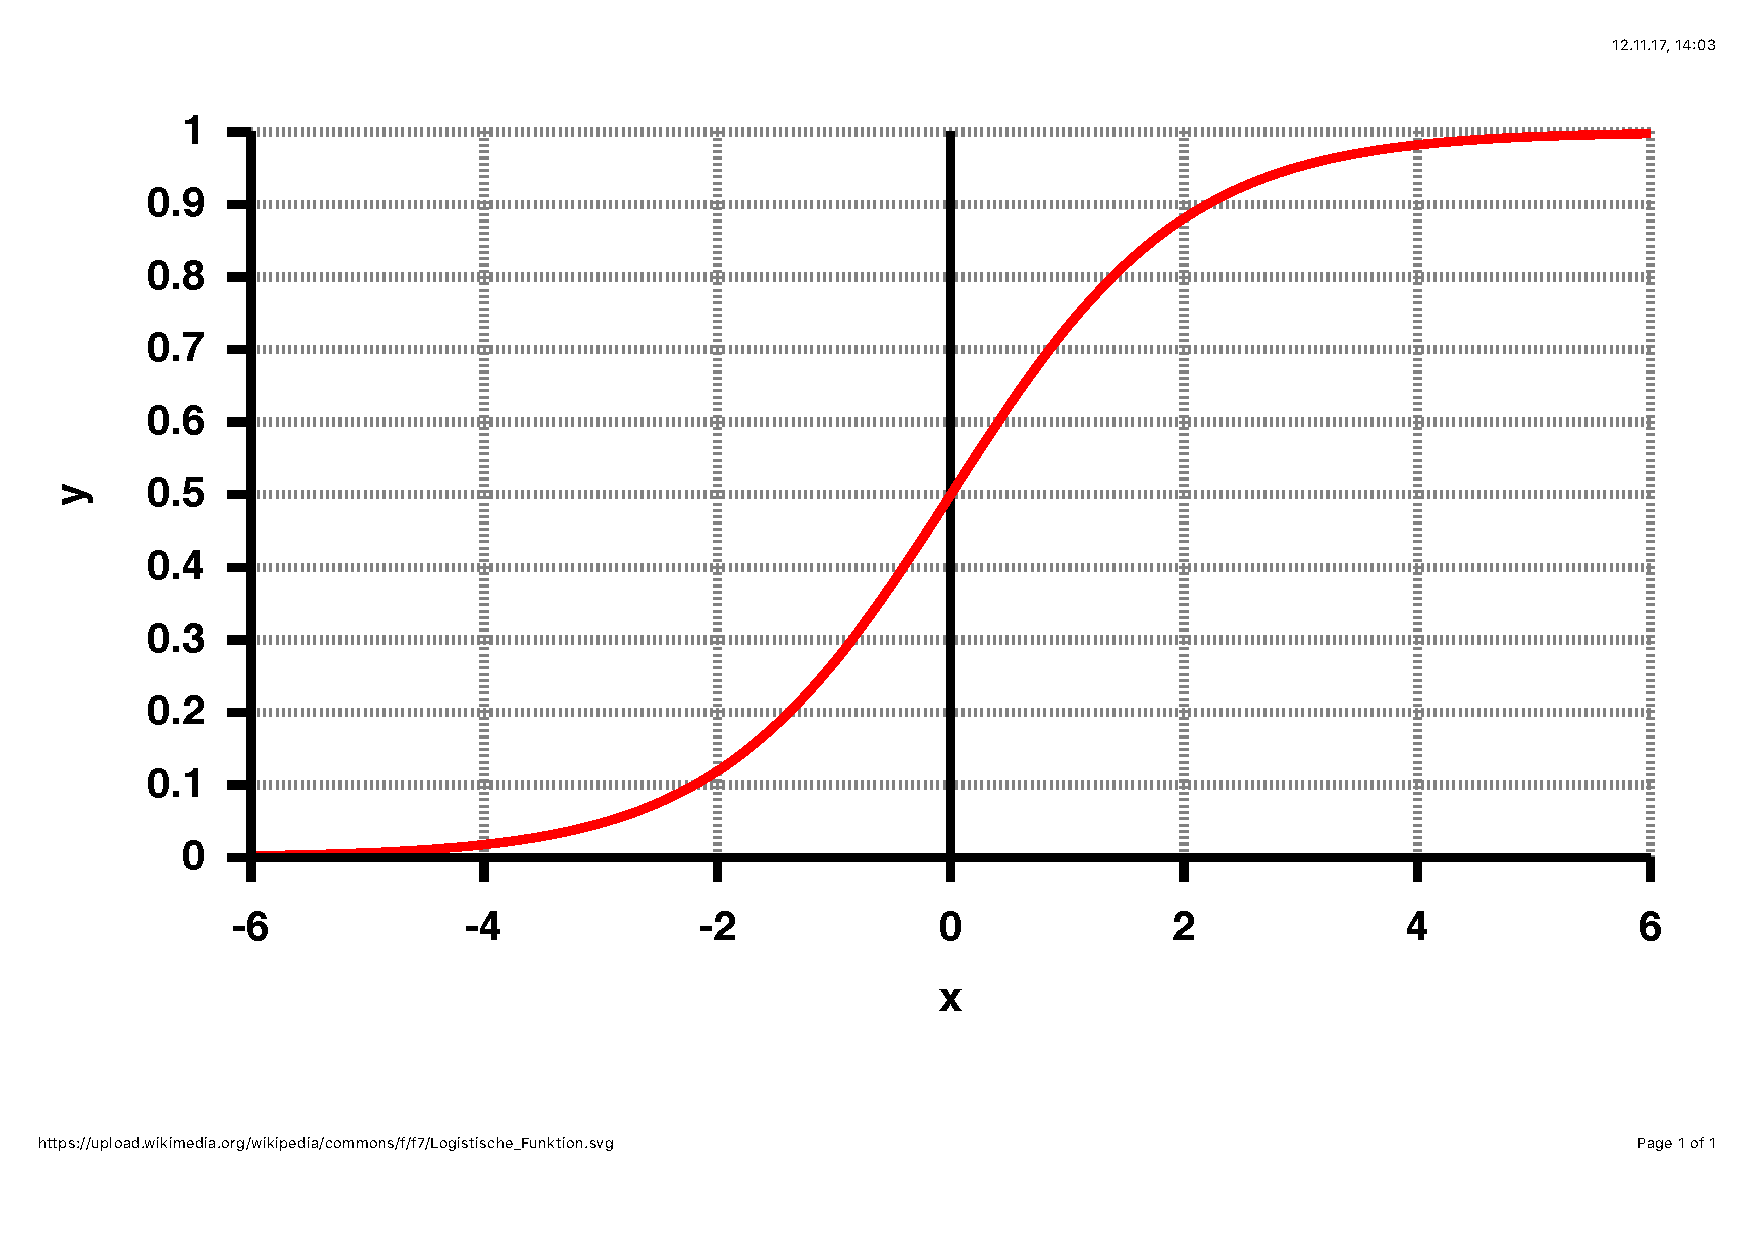
\includegraphics[scale=0.4]{img/grafik_markt.pdf} 
		\caption{Logisches Wachstum} \label{fig:abb24}
	\end{figure}
	
	Die aus dieser Formel resultierende Abnahmequote wird nun noch mit der angebotenen Menge und dem sog. \enquote{\texttt{Marketingboost}} multipliziert, was nachbildet, dass unattraktive Uhren, unabhängig von der angebotenen Menge, eher zu Ladenhütern werden als attraktivere und im Programm als \enquote{\texttt{Abnahmepotential}} bezeichnet wird. Bei schlechten Angeboten wird mit diesem Algorithmus errechnet, welcher Prozentteil des Angebots zu Ladenhütern wird und welcher im Gegenzug überhaupt verkaufbar ist. Ebenso wird Uhren mit größerem Abnahmepotential später ein gewisser Vorteil eingeräumt, da diese eine größere Präsenz in den Läden haben.
	\item Die drei Marktsegmente sollen sich gegenseitig beeinflussen
	\\ Um anzugeben, wie stark sich die Teilmärkte gegenseitig beeinflussen wurde davon ausgegangen, dass in der Ausgangslage die Kunden einem Segment zugeordnet werden können und so die unabhängigen Marktvolumina darstellen. Jedoch können Teile der Kundenbasis durch attraktive Angebote abgeworben werden. Dazu wird für jede Uhr der sog. \enquote{\texttt{volumeChange}} berechnet, bevor diese an die Teilmärkte übergeben wird. Bei guten Angeboten wird das Marktvolumen des korrespondierenden Teilmarktes um diesen \texttt{volumeChange} erhöht und die anderen Teilmarktvolumina um die Hälfte dieses Wertes verringert.
	\item Die Uhren im selben Marktsegment sollen sich gegenseitig beeinflussen
	\\ Damit berechnet werden kann, wie stark sich alle Uhren im selben Marktsegment gegenseitig beeinflussen werden alle Uhren aller Spieler zuerst in drei Listen sortiert, die dann jeweils den drei Teilmärkten übergeben werden. So ist es egal wie viele Uhren in einem Segment angeboten werden oder von wem, denn auch die eigenen Uhren sind als Konkurrenz zu sehen. In den Teilmärkten wird dann für jede Uhr die sog. \enquote{\texttt{konkurrenz}} berechnet, die Stückzahl aller konkurrierenden Uhren zu dem Preis der Ausgangsuhr. In dieser Rechnung wird jedoch bereits das in Punkt 3 berechnete Abnahmepotential statt der angebotenen Menge benutzt, das Preis-Leistungs-Verhältnis ist also bereits eingerechnet. Dabei ist eine Uhr definiert als eine Uhr, deren Preis (unabhängig vom Wert) innerhalb eines Preisspektrums zur Ausgangsuhr liegt. Dieses Spektrum ist definiert durch die beim Erstellen des Marktes angegebene Variable \texttt{impactRange}, ist die Differenz der Angebotspreise der beiden Uhren kleiner als das Produkt aus Angebotspreis der 2. Uhr mit diesem \texttt{impactRange}, zählen die Uhren als konkurrierend. Sind 2 Uhren in direkter Konkurrenz wird das \texttt{Abnahmepotential} zur \texttt{konkurrenz} addiert, nachdem es mit einem Faktor zwischen 1 und 0 multipliziert wurde, der kleiner wird je weiter auseinander die Preise liegen. Ist die gesamte \texttt{konkurenz} kleiner als das Marktvolumen zu dem Preis der Uhr ist der Markt nicht gesättigt und die Uhr kann alle beim \texttt{Abnahmepotential} berechneten Uhren verkaufen, sollte die \texttt{konkurrenz} größer sein, werden die Verkaufszahlen aller Uhren soweit gleichmäßig geschrumpft, dass das Marktvolumen nicht überschritten wird.
\end{enumerate}
Diese Marktsimulation hat zur Folge, dass Uhren die zu attraktiven Preisen angeboten werden bevorzugt werden, überteuerte Uhren jedoch nicht komplett Machtlos sind und mit schierer Masse Marktanteile erobern können. Ebenso kann durch attraktive Angebote die Käuferschaft von anderen Marktsegmenten abgeworben werden und so über den gesamten Markt Einfluss ausgeübt werden.

\newpage
\section{Klasse}
\begin{figure} [!h]
	\centering
	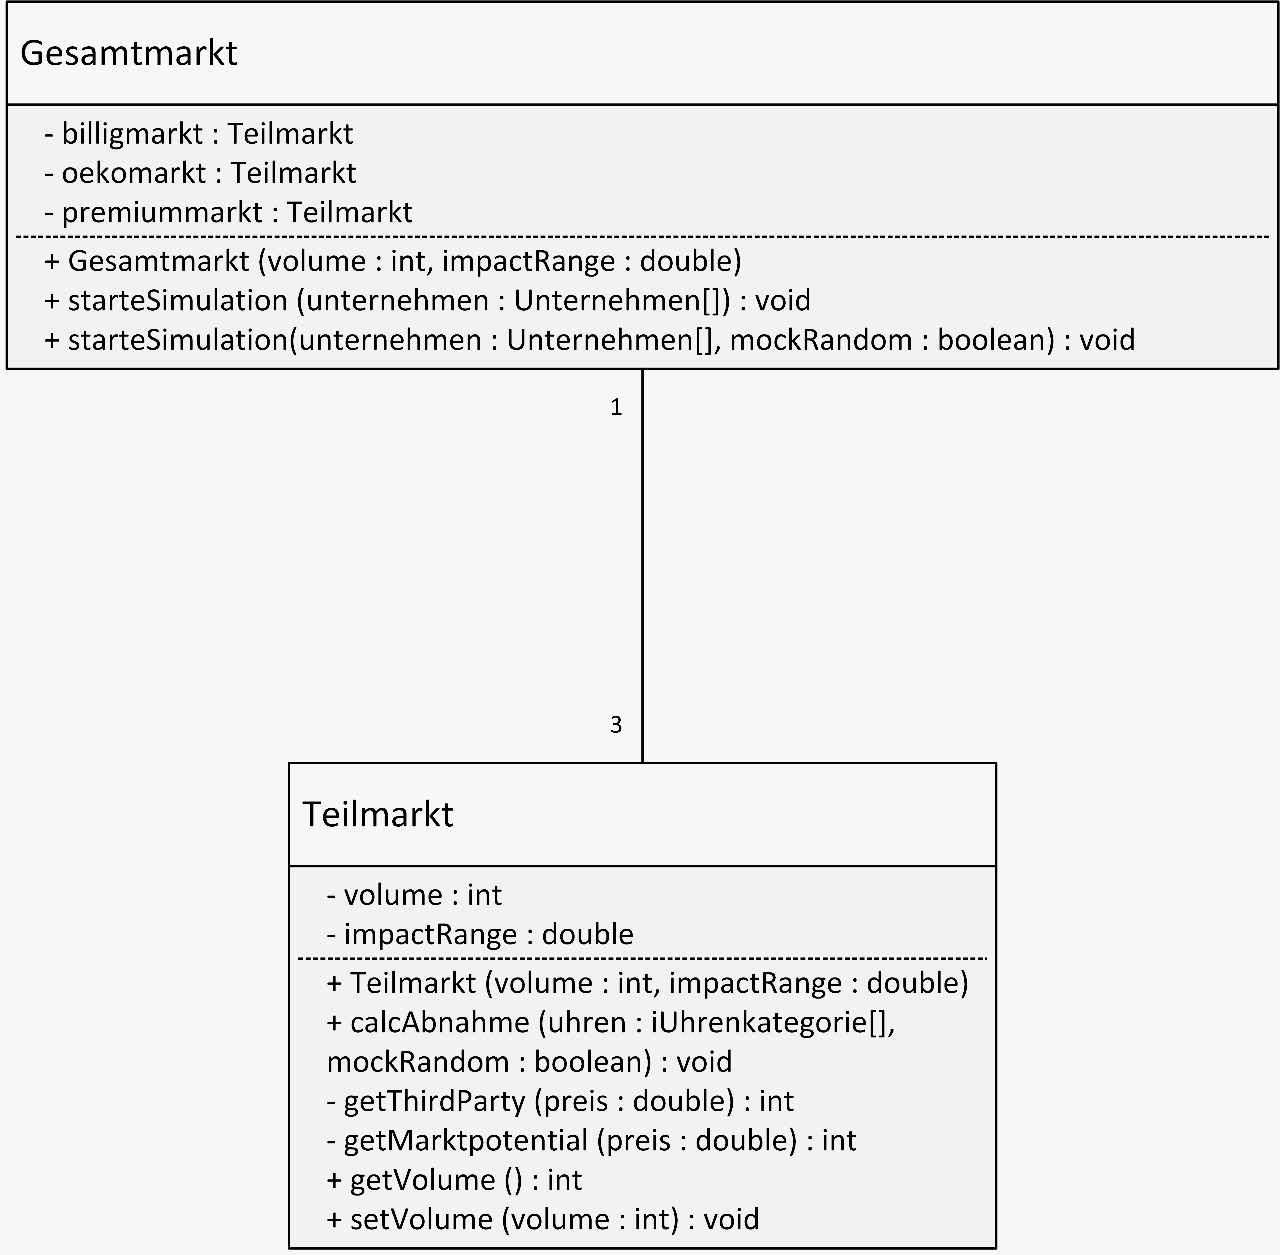
\includegraphics[scale=0.3]{img/Markt.jpeg} 
	\caption{Markt Klasse} \label{fig:25}
\end{figure}
